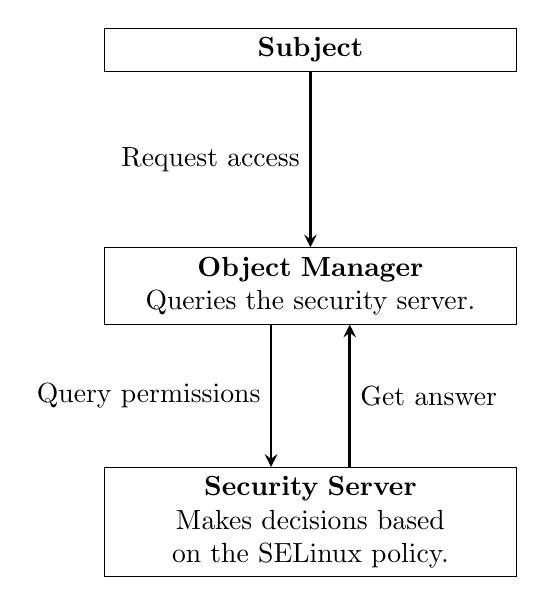
\begin{tikzpicture}
    \usetikzlibrary{calc}
    \tikzstyle{line} = [->,>=stealth, line width=1pt]
    \tikzstyle{rec} = [rectangle, draw=black, align=center, text width=5cm]

    \node(subject) [rec] {\textbf{Subject}};
    \node(objman) [rec, below of=subject, node distance=3cm] {\textbf{Object
    Manager}\\ Queries the security server.};
    \node(secser) [rec, below of=objman, node distance=3cm]
    {\textbf{Security Server}\\ Makes decisions based on the SELinux
    policy.};

    \draw[line] (subject) -- node[midway,left] {Request access} (objman);
    \draw[line] ([xshift=-0.5cm]objman.south) -- node[midway,left] {Query
    permissions} ([xshift=-0.5cm]secser.north);
    \draw[line] ([xshift=0.5cm]secser.north) -- node[midway,right] {Get
    answer} ([xshift=0.5cm]objman.south);
\end{tikzpicture}
